In this section, we introduce the first kind arithmetic expression space $\mathfrak{E}_1$, which provides a geometric framework for studying arithmetic expressions. We begin with motivating examples, establish the general framework, explore geometric propagation, and examine the relationship between grids and torsion in this space.

\subsection{Motivating examples}\label{subsec:motivexamples}

We present two analytic examples that are equivalent and belong to the class of spaces called the first kind arithmetic expression space $\mathfrak{E}_1$.

\subsubsection{Example 1: Upper Half Plane Model}

Consider the upper half plane ${\mathcal{H}: (x, y) \ | \ y > 0}$ equipped with the following inner product and metric:

$$
\mathbf{a} \cdot \mathbf{b} = \begin{bmatrix} a_x & a_y \end{bmatrix} \begin{bmatrix} \frac{1}{y^2} & 0 \\ 0 & \frac{1}{y^2} \end{bmatrix} \begin{bmatrix} b_x \\ b_y \end{bmatrix}
$$

$$
ds^2 = \frac{1}{y^2} (dx^2 + dy^2)
$$

On this space, we define an assignment field $a$ as follows:

\begin{equation}\label{eq:exmp1}
a = - \frac{x}{y}
\end{equation}

\begin{theorem}\label{thm:exmp1}
The assignment $a$ defined by formula \eqref{eq:exmp1} satisfies the flow equation \eqref{eq:flow}.
\end{theorem}

\begin{proof}
We begin with the differential of the assignment:
$$
da = d\left(-\frac{x}{y}\right) = \frac{xdy - ydx}{y^2} = -\frac{dx + ady}{y}
$$

The differential of arc length is:
$$
ds = \frac{\sqrt{dx^2 + dy^2}}{y}
$$

Therefore:
$$
\frac{da}{ds} = - \frac{dx + ady}{y} \cdot \frac{y}{\sqrt{dx^2 + dy^2}} = - \frac{dx + ady}{\sqrt{dx^2 + dy^2}}
$$

In the local coordinate system given by $(-1, 0)$ and $(0, -1)$ under the right-hand rule, we have:
$$
\cos \theta = \frac{-dx}{\sqrt{dx^2 + dy^2}} \quad \text{and} \quad \sin \theta = \frac{-dy}{\sqrt{dx^2 + dy^2}}
$$

Substituting these values:
$$
\frac{da}{ds} = \cos \theta + a \sin \theta
$$

This matches the flow equation \eqref{eq:flow} with $\mu=1$ and $\lambda=1$.
\end{proof}

We can verify that $a$ is an eigenfunction of the Laplacian operator:
$$
\Delta a = - y^2 \left(\frac{\partial^2 a}{\partial x^2} + \frac{\partial^2 a}{\partial y^2}\right) = y^2 \left(\frac{\partial}{\partial y} \left(\frac{\partial}{\partial y} \frac{x}{y}\right)\right) = 2a
$$

\subsubsection{Example 2: Horocycle-Based Coordinate System}

For our second example, we first introduce a horocycle-based coordinate system for hyperbolic surfaces. This global coordinate system consists of two orthogonal sets of circles: horocycles sharing the same ideal point, and geodesics perpendicular to these horocycles.

\begin{figure}[ht]
\centering
\resizebox{0.5\textwidth}{!}{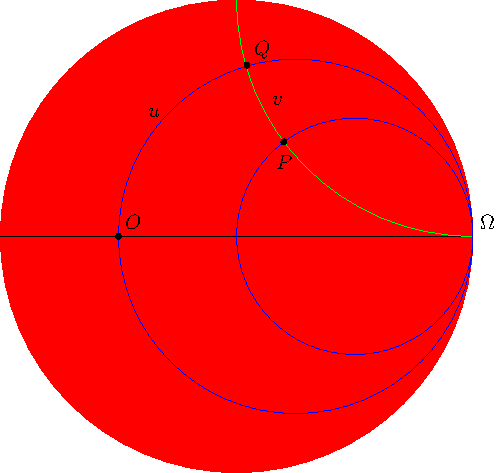
\includegraphics{images/11-horocyclebased}}
\caption{A horocycle-based coordinate system on the Poincaré disc. Blue curves are horocycles tangent at ideal point $\Omega$, green lines are perpendicular geodesics.}\label{fig:horocyclecoord}
\end{figure}

On the Poincaré disc $\mathcal{P}$, the coordinates of a point $P$ are given by $(u,v)$, where:
\begin{itemize}
\item $u$ is the signed length of $OQ$
\item $v$ is the signed length of $QP$
\item The signs follow the right-hand rule and orientation relative to the ideal point $\Omega$
\end{itemize}

We equip this coordinate system with the inner product:
$$
\mathbf{a} \cdot \mathbf{b} = \begin{bmatrix} a_u & a_v \end{bmatrix} \begin{bmatrix} e^{-2v} & 0 \\ 0 & 1 \end{bmatrix} \begin{bmatrix} b_u \\ b_v \end{bmatrix}
$$

And the metric:
$$
ds^2 = e^{-2v} du^2 + dv^2
$$

The Laplacian in this coordinate system is:
$$
\Delta = e^{2v} \frac{\partial^2}{{\partial u}^2} + \frac{\partial^2}{{\partial v}^2} - \frac{\partial}{\partial v}
$$

In this coordinate system, we define an assignment:

\begin{equation}\label{eq:exmp2}
a = u e^{-v}
\end{equation}

\begin{theorem}\label{thm:exmp2}
The assignment $a$ defined by formula \eqref{eq:exmp2} satisfies the flow equation \eqref{eq:flow}.
\end{theorem}

\begin{proof}
We establish this result by showing that examples 1 and 2 are equivalent through a Möbius transformation. Consider the complex representation of the upper half plane:
$$
z = x + yi
$$

The Möbius transformation mapping the upper half plane to the Poincaré disc is:
$$
z \mapsto \frac{z-i}{z+i}
$$

\begin{figure}[ht]
\centering
\resizebox{0.8\textwidth}{!}{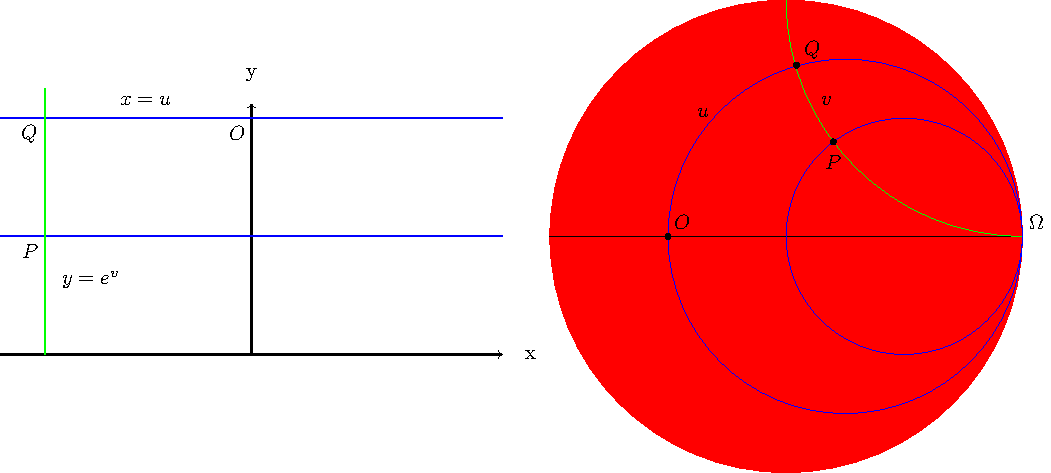
\includegraphics{images/12-proofbymapping}}
\caption{Mapping between the upper half plane and Poincaré disc models}\label{fig:mapping}
\end{figure}

This transformation maps horizontal lines in $\mathcal{H}$ to horocycles sharing the ideal point $\Omega = 1$ in $\mathcal{P}$, and vertical geodesics in $\mathcal{H}$ to perpendicular geodesics in $\mathcal{P}$.

Expressed in the target coordinate system, this transformation gives:
$$
\begin{cases}
x = u\\
y = e^v \\
\end{cases}
$$

Substituting into the assignment from Example 1:
$$
a = -\frac{x}{y} = -\frac{u}{e^v} = -u e^{-v}
$$

Since the Möbius transformation is conformal and preserves the flow equation, and considering the orientation change, we have $a = u e^{-v}$ satisfying the flow equation.
\end{proof}

As in Example 1, we can verify that $a$ is an eigenfunction of the Laplacian:
$$
\Delta a = e^{2v} \frac{\partial^2(u e^{-v})}{{\partial u}^2} + \frac{\partial^2(u e^{-v})}{{\partial v}^2} - \frac{\partial(u e^{-v})}{\partial v} = 2a
$$

These two examples, arising from the same geometric setting but in different coordinate systems, demonstrate the fundamental properties of the first kind arithmetic expression space.

\subsection{General framework of $\mathfrak{E}_1$ space}\label{subsec:generalframework}

Building on the motivating examples, we now establish a general framework for the first kind arithmetic expression space $\mathfrak{E}_1$. 

Consider the upper half plane $\mathcal{B}$:
$$
\{\mathcal{B}: (x, y) | y > 0 \}
$$

equipped with an inner product and metric parameterized by constants $\mu$ and $\lambda$:

$$
\mathbf{a} \cdot \mathbf{b} = \begin{bmatrix} a_x & a_y \end{bmatrix} \begin{bmatrix} \frac{1}{\mu^2 y^2} & 0 \\ 0 & \frac{1}{\lambda^2 y^2} \end{bmatrix} \begin{bmatrix} b_x \\ b_y \end{bmatrix}
$$

$$
ds^2 = \frac{1}{y^2}\left(\frac{dx^2}{\mu^2} + \frac{dy^2}{\lambda^2}\right)
$$

The assignment function in this general framework remains:

\begin{equation}\label{eq:genassignment}
a = - \frac{x}{y}
\end{equation}

This defines the first kind arithmetic expression space $\mathfrak{E}_1$, characterized by the following theorem:

\begin{theorem}\label{thm:generalE1}
The assignment $a$ given by \eqref{eq:genassignment} satisfies the flow equation \eqref{eq:flow} with parameters $\mu$ and $\lambda$, independent of the specific values of these generators.
\end{theorem}

\begin{proof}
The differential of the assignment is:
$$
da = d\left(-\frac{x}{y}\right) = \frac{xdy - ydx}{y^2} = -\frac{dx + a dy}{y}
$$

The differential of arc length is:
$$
ds = \frac{1}{y}\sqrt{\frac{dx^2}{\mu^2} + \frac{dy^2}{\lambda^2}}
$$

Therefore:
$$
\frac{da}{ds} = - \frac{dx + a dy}{y} \cdot \frac{y}{\sqrt{\frac{dx^2}{\mu^2} + \frac{dy^2}{\lambda^2}}} = -\frac{dx + a dy}{\sqrt{\frac{dx^2}{\mu^2} + \frac{dy^2}{\lambda^2}}}
$$

In the local coordinate system given by $(-1, 0)$ and $(0, -1)$ according to the right-hand rule:

$$
\cos \theta = \frac{-\frac{dx}{\mu}}{\sqrt{\frac{dx^2}{\mu^2} + \frac{dy^2}{\lambda^2}}} \quad \text{and} \quad \sin \theta = \frac{-\frac{dy}{\lambda}}{\sqrt{\frac{dx^2}{\mu^2} + \frac{dy^2}{\lambda^2}}}
$$

Substituting these values:
$$
\frac{da}{ds} = \mu \cos \theta + a \lambda \sin \theta
$$

This matches the flow equation \eqref{eq:flow} with the given parameters $\mu$ and $\lambda$.
\end{proof}

The $\mathfrak{E}_1$ space is characterized by its connection to hyperbolic geometry and the property that the assignment function $a = -x/y$ is an eigenfunction of the Laplacian with eigenvalue 2. This space provides a natural geometric framework for studying arithmetic expressions, particularly those involving addition and multiplication operations.

\subsection{Geometric propagation}\label{subsec:geompropagation}

The flow equation in the $\mathfrak{E}_1$ space can be interpreted as describing the propagation of arithmetic expressions. This interpretation builds on the propagation method discussed in Section \ref{subsec:propagation-method}.

In the $\mathfrak{E}_1$ space, paths along constant $x$ (vertical lines in the upper half plane) correspond to multiplication operations, while paths along constant $y$ (horizontal lines) correspond to addition operations. The assignment value $a = -x/y$ propagates according to the flow equation as we move along these paths.

The propagation can be visualized as wavefronts emanating from sources in the upper half plane. Points with the same assignment value form equipotential curves, and the flow equation governs how these wavefronts evolve geometrically.

From equation \eqref{eq:gradevo5}, we recall that along the gradient direction ($\phi=0$) starting from $a_0=0$:
\begin{equation}
a = \pm \frac{\mu}{\lambda} \sinh(\lambda s)
\end{equation}

This resembles the formula for the circumference of a circle in hyperbolic space with curvature $-\lambda^2$:
\begin{equation}
C = \frac{2\pi}{\lambda} \sinh(\lambda s)
\end{equation}

This parallel suggests that the assignment $a$ propagates like expanding concentric circles in hyperbolic space, with the zero assignment line serving as the collection of centroids from which these circles emanate.

The dual perspective of propagation and evaluation provides a powerful framework for understanding arithmetic expressions geometrically:
1. Evaluation of an expression follows paths through the $\mathfrak{E}_1$ space
2. Different evaluation orders correspond to different paths with the same endpoints
3. The flow equation ensures that the final value is independent of the path taken (for evaluable expressions)

\subsection{Grids and torsion}\label{subsec:gridsandtorsion}

The addition-multiplication grid introduced in Section \ref{subsec:meshgrid} has a natural representation in the $\mathfrak{E}_1$ space. The grid consists of two families of orthogonal curves:
1. Addition curves (blue lines): paths of constant $y$ in the upper half plane
2. Multiplication curves (green lines): paths of constant $x/y$ ratio in the upper half plane

The grid structure allows us to visualize and analyze the arithmetic torsion discussed in Section \ref{subsec:generated-structure}.

\begin{figure}[ht]
    \centering
    \resizebox{0.8\textwidth}{!}{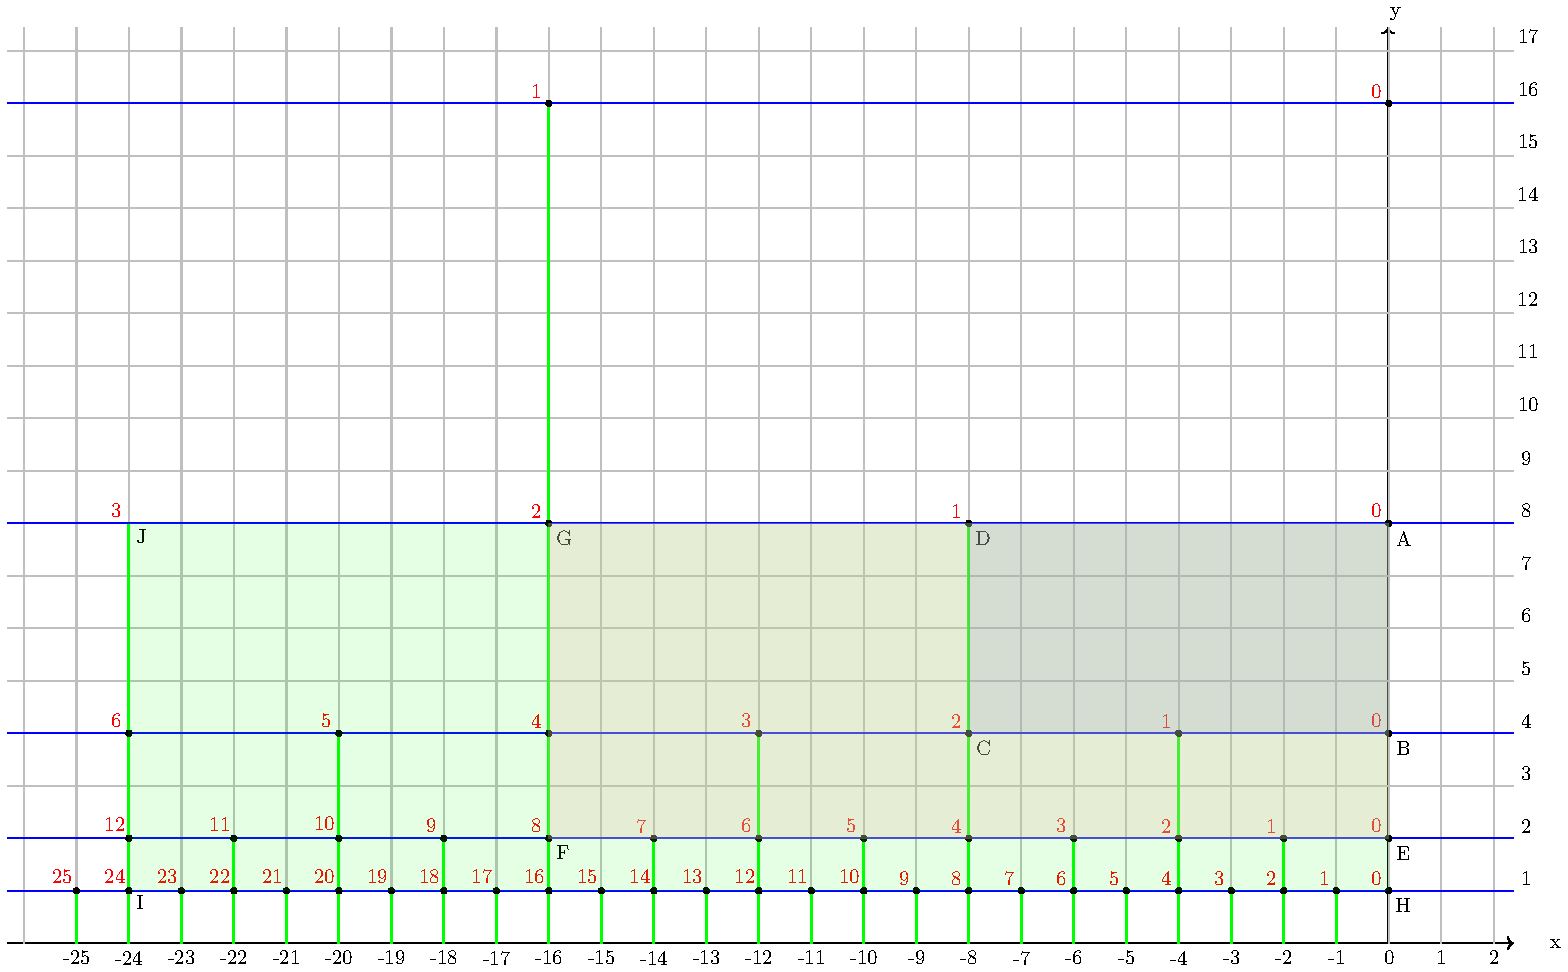
\includegraphics{images/17-area-formula}}
    \caption{Illustration of the relationship between area and arithmetic torsion}\label{fig:area-formula}
\end{figure}

Figure \ref{fig:area-formula} illustrates the connection between the area enclosed by grid paths and the arithmetic torsion. Consider the arithmetic torsion for different path combinations:

For a single step:
\begin{equation}
    x \times 2 + 1 - (x + 1) \times 2 = -1
\end{equation}

For two steps:
\begin{equation}
    x \times 4 + 2 - (x + 2) \times 4 = -6
\end{equation}

For three steps:
\begin{equation}
    x \times 8 + 3 - (x + 3) \times 8 = -21
\end{equation}

These values (-1, -6, -21) correspond to the areas of the enclosed regions in the grid:
- The quadrilateral $ABCD$ has area 1 (a single unit cell)
- The region $AEFG$ has area 6 (six unit cells)
- The region $AHIJ$ has area 21 (twenty-one unit cells)

This connection can be formalized through the area formula derived in Section \ref{subsec:descartes-coordinate}:
\begin{equation}
    d\tau = \mu \lambda du dv
\end{equation}

Where $d\tau$ is the differential of arithmetic torsion, and $du dv$ represents the area element in the arithmetic coordinate system.

The relationship between arithmetic torsion and area aligns with the concept of curvature in differential geometry. Just as curvature measures how much a surface deviates from being flat, arithmetic torsion measures how much arithmetic expressions deviate from being commutative. The $\mathfrak{E}_1$ space provides a geometric framework where this deviation is directly related to areas in the addition-multiplication grid.
